\documentclass[main.tex]{subfiles}

\begin{document}

Since Rosenblatt proposed the term perceptron in 1957,
many machine learning algorithms have been developed,
such as support vector machine, and deep learning.
Today, the most commonly used method is deep neural networks that have a lots of parameters to tune, for example, ResNet and Transformer
based on a powerful compute equipment and a large dataset.
However, although these methods are very powerful, the following problems exist.

\begin{itemize}
	\item Consumption of enormous computational resources
	\item Requires a large amount of training data
	\item Take a long time to train
	\item Easily overfitted
\end{itemize}

Hence, it is difficult to use a huge model in situations
where computational resources are insufficient and data are not enough,
and instead, a small model may be a better choice.
Small models are generally faster than large models
and are learned well enough with even small dataset.

In this paper, we compared the accuracy and speed of some algorithms,
and investigated suitable model for use in computer vision tasks.

Hand-written digit dataset (MNIST) includes 1,797 grayscale images whose width and height are 8 respectively.
Each image contains one of the numbers from 0 to 9.
All input data is expressed as a matrix composed of values between 0 and 16.
To be more specific, in an image, pixels without digits are represented by numbers close to zero,
and pixels with digits are represented by numbers close to 16.
Our goal is to use this dataset to build a model that predicts which of the numbers an image is.
Fig. \ref*{edafig}--(b) shows that the number of samples in each class is nearly equal, so that we do not need to care about the processing of the imbalanced dataset.
And in Fig. \ref*{edafig}--(c), numbers are mostly located in the middle of the image.

The remainder of the paper is organized as follows.
Section II introduces how we set up and trained models.
In Section III, each model is compared based on the results of the experiment.
Finally, we conclude the paper in Section IV.

\begin{figure}[H]
	\centering
	\subcaptionbox{Sample Data}[.3\textwidth] {
		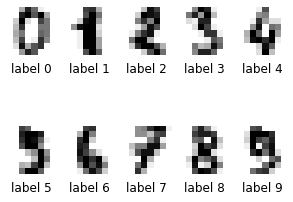
\includegraphics[scale=0.5]{img/eda/data_examples.png}
	}
	\subcaptionbox{Data Distribution}[.3\textwidth] {
		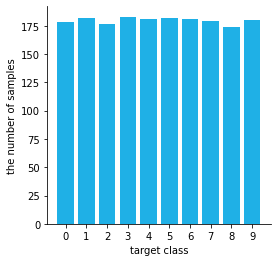
\includegraphics[scale=0.45]{img/eda/data_dist.png}
	}
	\subcaptionbox{Mean Image}[.3\textwidth] {
		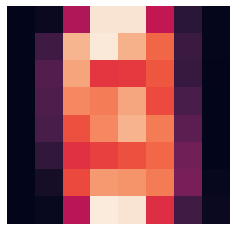
\includegraphics[scale=0.5]{img/eda/data_mean.png}
	}
	
	\caption{(a) Sample images for each class. (b) The number of samples in each class. (c) Image where $(i, j)$ pixel is an average of $(i, j)$ pixels from all images.}
	\label{edafig}
\end{figure}

\end{document}
